\subsection{Vergleich vorhandener Systeme}
\subsubsection{CS50 der Harvard University}
\paragraph{Allgemeines}
CS50 ist die ursprüngliche Bezeichnung eines Lernkurses über Informatik,
welcher von der Harvard University ins Leben gerufen wurde und weiterhin
betreut wird. Der Kurs wurde aufgrund seines Erfolgs digitalisiert und wird nun
als CS50x auf der Lernplattform edX angeboten. Folgende Recherchen und Aussagen
sind jeweils immer auf die Online-Version CS50x bezogen.

Der Kurs CS50 lehrt Schüler\footnote{Aus Gründen der besseren Lesbarkeit wird
in der gesamten Arbeit auf die gleichzeitige Verwendung der Sprachformen
männlich, weiblich und divers (m/w/d) verzichtet. Sämtliche
Personenbezeichnungen gelten gleichermaßen für alle Geschlechter. Ist eine
spezifische Geschlechtergruppe gemeint, wird das entsprechende Adjektiv
vorangestellt (z.B. \glqq männliche Studenten\grqq)} die Grundlagen der
Informatik. Dabei werden diverse Programmierübungen abgefragt. Aufgrund der
hohen Anzahl an Teilnehmern besitzt der Kurs ein automatisiertes Abgabe- und Benotungssystem.

Das System hinter CS50 wird mittlerweile vielfältig eingesetzt und wurde zu
einem universalen Online-Lernsystem erweitert. Jeder kann sich durch eine
Authentifizierung über die Plattform GitHub im Abgabesystem von CS50 einloggen
und eigene Kurse erstellen. \parencite{cs50}

\newpage
\paragraph{Ablauf für Studierende}
Dem Teilnehmer wird jede Woche ein neues Kapitel präsentiert. Er kann sich dabei
sowohl durch ein Vorlesungsvideo, als auch durch geschriebene Materialien über
das Thema der Woche informieren. Mit Beginn der Woche bekommt der Teilnehmer
neben den Materialien auch Programmieraufgaben, welche er mit dem vorher
genannten System bearbeiten kann. \parencite{cs50-edx}

Die Programmieraufgaben können wahlweise über die, auf AWS Cloud9 basierenden,
Online-Entwicklungsumgebung \glqq CS50-IDE\grqq{} von Harvard oder in jeder
anderen beliebigen Entwicklungsumgebung der Wahl bearbeitet werden. Dies
wird durch die Architektur des Systems ermöglicht. Jede Funktionalität der
Automatisierung geschieht durch Kommandozeilen-Tools. Dieses System hat den
Vorteil, dass es unabhängig von der eingesetzten IDE funktioniert, es wird
lediglich ein Terminal mit den jeweiligen Tools benötigt. \parencite{cs50-ide}

Vor der Abgabe der endgültigen Lösung mit dem sogenannten Werkzeug
\glqq submit50\grqq{}, ist es möglich den Code mit einem weiteren Werkzeug
namens \glqq check50\grqq{} überprüfen zu lassen. Außerdem gibt es viele weitere
Werkzeuge, ein Beispiel hierfür ist \glqq style50\grqq{}, welches die Qualität
und den Style des Programmcodes überprüft und bewertet. \parencite{submit50}

\paragraph{Architektur}
Die Harvard University hält den Aufbau von CS50 weitestgehend transparent.
Viele der eingesetzten Werkzeuge sind öffentlich als Open-Source-Projekte unter
der GitHub-Organisation \glqq CS50\grqq{} zu finden \parencite{cs50-github}. Darunter
befinden sich unter anderem folgende Projekte:
\begin{itemize}
\item submit50: Abgabe von Code
\item check50: Funktionalitätstests des Codes
\item render50: Erzeugung von .PDF-Dateien aus Code
\item ide50: Online-Entwicklungsumgebung
\item style50: Überprüfung der Code-Qualität
\item compare50: Plagiatserkennung von abgegebenen Projekten
\item server50: Webserver
\end{itemize}

\newpage

In Abbildung \ref{fig:cs50-architektur} ist der Aufbau der Lernplattform CS50
vereinfacht grafisch dargestellt. Die Rechtecke und Menschen sind die
beteiligten Komponenten. Die Pfeile zwischen den Komponenten beschreiben die
verbindende Relation. Von der \glqq CS50-Programm\grqq-Komponente ausgehende gestrichelte Pfeile zeigen, je nach ausgeführtem Befehl, mögliche Relationen.

\begin{figure}[h]
    \centering
    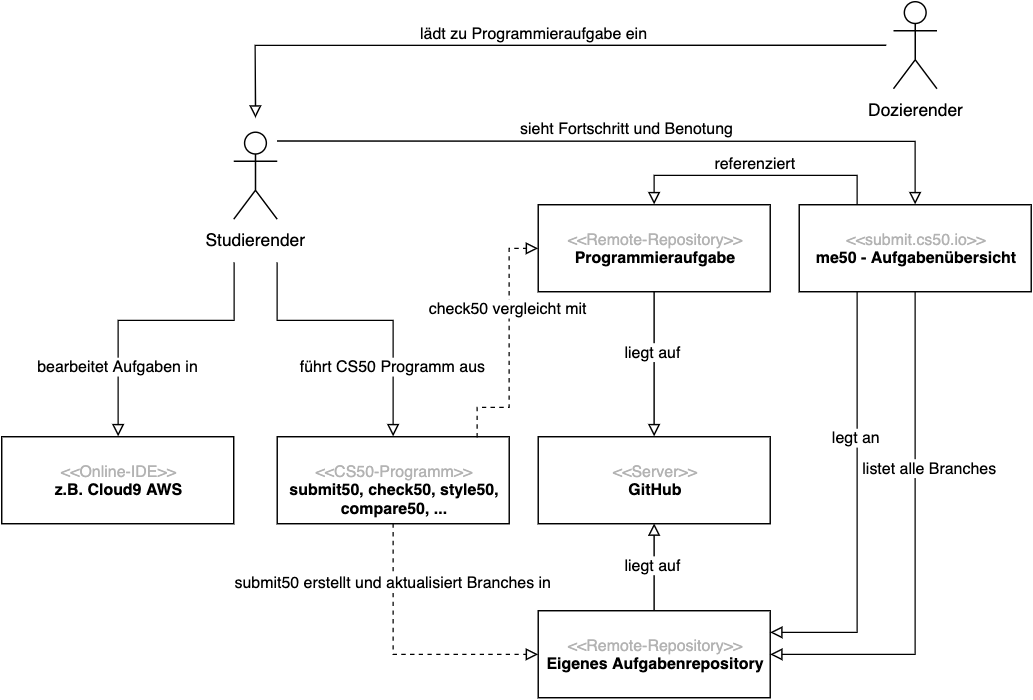
\includegraphics[width=\textwidth]{cs50-architektur}
    \caption{CS50 Architektur}
    \bildquelle{Eigene Darstellung}
    \label{fig:cs50-architektur}
\end{figure}

\paragraph{Probleme beim Einsatz für die OTH}
Die Toolchain von CS50 wäre adäquat für den Einsatz an der OTH-Regensburg.
Eines der Projekte ist aktuell noch nicht Open-Source: die Website zur
Erstellung von neuen Kursen, Abgaben und Mitgliederverwaltung. Dieses Projekt
ist essenziell für die Verwendung der Werkzeuge an der Regensburger Hochschule.
Nach Rücksprache mit Herrn Carter Zenke der Harvard University ist ein Neuaufbau
dieser Website mit einhergehender Veröffentlichung als Open-Source-Projekt
gerade in Planung. Einen genauen öffentlichen Zeitplan hierfür gibt es aktuell
nicht. Infolgedessen ist ein Einsatz des CS50-Systems an der OTH zum heutigen
Datum nicht möglich.

\newpage
\subsubsection{Code FREAK der Fachhochschule Kiel}\label{code-freak}
\paragraph{Allgemeines}
Code FREAK ist eine All-in-one-Lösung für Online-Programmieraufgaben mit
automatisiertem Feedback. Die von der Hochschule Kiel entwickelte
Open-Source-Software soll den Einstieg in eine digitale Lernumgebung einfach
machen. Die Zielgruppe von Code FREAK bezieht sich hierbei explizit auf
Universitäten und Einrichtungen einer höheren Bildung.
\parencite{codefreak-startseite}

Des Weiteren wirbt Code FREAK mit einer LMS-Integration. LMS ist die englische
Abkürzung für Learning Management System (dt. Lernplattform). Viele Schulen und
Universitäten verwenden bekannte LMS-Systeme, wie Moodle, um Kurse, Fächer und
Studierende zu verwalten \parencite{moodle}.
Dies hat den Vorteil, dass Studierende kein extra Nutzerkonto für Code FREAK
anlegen müssen. Sie können sich direkt mit ihrem gewohnten Zugang anmelden.

\paragraph{Ablauf für Studierende}
Studierende können nach Anmeldung am System, an für sie sichtbaren Kursen
(Assignments) teilnehmen. Dies geschieht meist durch einen vom Dozenten
generierten Einladungslink. Jedes Assignment kann mehrere Aufgaben (Tasks)
enthalten. Die einzelnen Aufgaben können dann entweder über die integrierte
Online-Entwicklungsumgebung, durch Hochladen der Lösung, oder durch die Angabe
eines Git-Repository-Links bearbeitet werden.

Mit dem Klick auf den Knopf \glqq Start Evaluation\grqq{} wird hochgeladene
Lösung der Aufgabe überprüft. Die Ergebnisse der einzelnen Test-Schritte können
dann in einem weiteren Tab eingesehen werden. Wenn alle Tests der Aufgabe
bestanden wurden, wird der Task mit einem grünen Haken versehen. So sieht der
Schüler in der Assignment-Ansicht auf einen Blick, welche Aufgaben er bereits
gelöst hat.

\paragraph{Architektur}
Code FREAK wird als fertiger Docker-Container ausgeliefert. Docker ist eine
Software um mithilfe von Containervirtualisierung einzelne Anwendungen
voneinander zu isolieren. Durch die Containervirtualisierung werden unter
anderem viele Abhängigkeits- und Einrichtungsprobleme beseitigt. Der Container
enthält alle Bibliotheken und Abhängigkeiten, die die Software für die Laufzeit
benötigt \parencite{docker}. Docker entstand auf Basis von Linux-Containern, welche
ein oder mehrere Prozesse vom restlichen System isolieren können 
\parencite{linux-container}.

Durch diese Handhabung kann Code FREAK mit nur einem Befehl in der
Kommandozeile installiert und gestartet werden. Die Software benötigt
grundsätzlich nur einen Container. Benutzt ein Studierender jedoch die
integrierte Online-Entwicklungsumgebung (Online-IDE), muss für jede Instanz ein
zusätzlicher Container mit der Laufzeitumgebung der IDE gestartet werden. Jeder
weitere Container benötigt weiteren Arbeitsspeicher.

\paragraph{Probleme beim Einsatz für die OTH}
Beim Einsatz von Code FREAK an der Hochschule Regensburg gibt es einige
Probleme. Das erste Problem bezieht sich auf den vorher erwähnten
Arbeitsspeicher. Die Praxis zeigt, dass eine Instanz der Online-IDE schon nach
wenigen Dateien ~3 Gigabytes an Arbeitsspeicher verwendet. Um eine reibungslose
und parallele Nutzung für alle Studierende des Kurses gewährleisten zu können,
werden dementsprechend sehr hohe Serverkosten fällig. 
\parencite{codefreak-memory-problem}

Eine weitere Hürde ist die Stabilität der Software. Code FREAK befindet sich,
Stand heute, mitten in der Entwicklung, weshalb einige Funktionen und Features
noch nicht ordnungsgemäß funktionieren. Darunter die vorher geworbene
LMS-Integration \parencite{codefreak-docs}. Zum heutigen Zeitpunkt ist LDAP die
einzige Möglichkeit sich mit dem System zu authentifizieren. Ein eigenes
Anmeldeverfahren gibt es nicht.

LDAP steht für \glqq Lightweight Directory Access Protocol\grqq{} und ist ein
Netzwerkprotokoll zur Durchführung von Abfragen und Änderungen in einem 
verteilten Verzeichnisdienst. LDAP ist der De-facto Industriestandard für
Authentifizierung und Autorisierung. \parencite{ldap}

Der Kurs Digital Skills soll den Teilnehmern einen Überblick über den
Arbeitsalltag eines Informatikers geben. Dazu gehört unter anderem die
Kommandozeile. Eine Anforderung der Lernplattform ist deshalb, dass man
(optional) neue Aufgaben herunterladen und Lösungsversuche über Befehle in der
Kommandozeile testen und abgeben kann. In Code FREAK kann man Aufgaben lediglich
über die Oberfläche testen und abgeben.

\newpage
\subsubsection{GitHub Classroom}
\paragraph{Allgemeines}
% TODO: GitHub Classroom kann auch LMS Integration
GitHub Classroom ist ein weiterer Kandidat für den Einsatz an der
Hochschule Regensburg. Die Plattform ermöglicht die automatisierte
Erstellung von Repositories auf GitHub. Außerdem hilft Classroom dabei,
Aufgabenvorlagen und dazugehörige Abgaben einfach zu verwalten und automatisch
zu benoten. Dabei enthalten die von GitHub Classroom erstellten
Aufgaben-Repositories bereits vorkonfigurierte Zugriffskontrollen. \parencite{github-classroom-startseite}

\paragraph{Ablauf für Studierende}
Studierende bekommen pro Programmieraufgabe einen Einladungslink.
Nach Annahme der Einladung wird pro Studierenden automatisch ein Repository für
die jeweilige Aufgabe angelegt. Dieses Repository enthält die Vorlage,
welche zum Bearbeiten der Aufgabe benötigt wird.

Sobald der Studierende eine Lösung zur Korrektur abgeben möchte, kann er per
Push die Änderungen in das Remote-Repository hochladen. Je nach Konfiguration
der Aufgabe starten daraufhin serverseitig ein oder mehrere Tests. Wenn alle
Tests bestanden sind, hat der Studierende die Aufgabe erfolgreich abgeschlossen.

\paragraph{Architektur} % TODO: Zitieren?
GitHub Classroom ist ein Bildungsservice der Firma GitHub Inc. und ist Stand
heute kostenfrei \parencite{github-classroom-kostenlos}. Die Software basiert
auf der Automatisierung von Repositories. Jeder bei GitHub registrierte Nutzer,
kann einen sogenannten \glqq Classroom\grqq erstellen und darin Aufgaben auf
Basis vorhandener öffentlichen GitHub-Repositories erstellen.

\paragraph{Probleme beim Einsatz für die OTH}
Es gibt keine Möglichkeit das System von GitHub Classroom auf einen lokalen
Git-Server zu replizieren. Aufgrund dessen schafft man sich durch die
Verwendung von Classroom eine externe Abhängigkeit an GitHub. Dies kann unter
Umständen zu erheblichen Problemen führen, wenn der Dienst beispielsweise
nicht erreichbar oder aufgelöst wird. Ersteres ist durch die Größe und
Infrastruktur des Unternehmens nicht (häufig) zu erwarten.

Eine weitere Hürde ist der Bedarf an weiterer Software. GitHub Classroom alleine
ist nicht ausreichend, um als vollständige Lernplattform für den Kurs Digital
Skills geeignet zu sein. Hier bietet es sich an, eine eigene statische Website
mit Anleitungen und Erklärungen zu bauen, welche dann jeweils auf Classroom
Einladungslinks verweist. Als Online-Entwicklungsumgebung kann der Dienst Replit
verwendet werden. In Replit ist es möglich, ein vorhandenes Git-Repository als
Template für eine neue Umgebung zu verwenden. Dieses Template könnte
Wrapper-Programme für den git-Workflow enthalten. Der Vorteil daran:
Studierende bekommen erste Erfahrungen mit der Kommandozeile, müssen jedoch
keine komplexen Git-Kommandos absetzen.

\subsubsection{Bewertung und Entscheidung der vorhandenen Systeme}
Die folgende Abbildung \ref{fig:systemvergleich} visualisiert die erläuterten
Systeme und bewertet diese anhand der vorher definierten Anforderungen (siehe 
Kapitel \ref{anforderungsanalyse}). Wie man der Grafik entnehmen kann,
repräsentieren alle blau hinterlegten Zeilen die nichtfunktionalen
Anforderungen. Alle rosa hinterlegten Zeilen wiederum repräsentieren die
funktionalen Anforderungen aus der Sicht des Teilnehmers. Der letzte Teil,
welcher gelb hinterlegt ist, spiegelt schließlich die funktionalen Anforderungen
aus der Sicht der Lehrenden wider.

Die erste Spalte enthält die Namen der Anforderungen, während die zweite Spalte
eine jeweilige Gewichtung der Anforderung enthält. Der valide Bereich dieser
Spalte befindet sich zwischen, einschließlich 0,00 und einschließlich 1,00. Eine
1,00 bedeutet, dass die Anforderung sehr wichtig ist. Je niedriger der Wert,
desto unwichtiger die Anforderung.

Die Spalten drei, vier und fünf enthalten die Benotungen der Systeme zu den
Anforderungen. Hierbei gilt ähnlich wie bei der Gewichtung: je höher der Wert,
desto besser. Der valide Bereich befindet sich hier jedoch zwischen 0,0 und 3,0.
Der Wert 0 bedeutet, dass das Feature nicht vorhanden ist, oder nicht zutrifft.
Die Spalten enthalten hierbei das Ergebnis der Multiplikation aus der Bepunktung
mit der in der zweiten Spalte enthaltenen Gewichtung.

\begin{figure}[H]
    \centering
    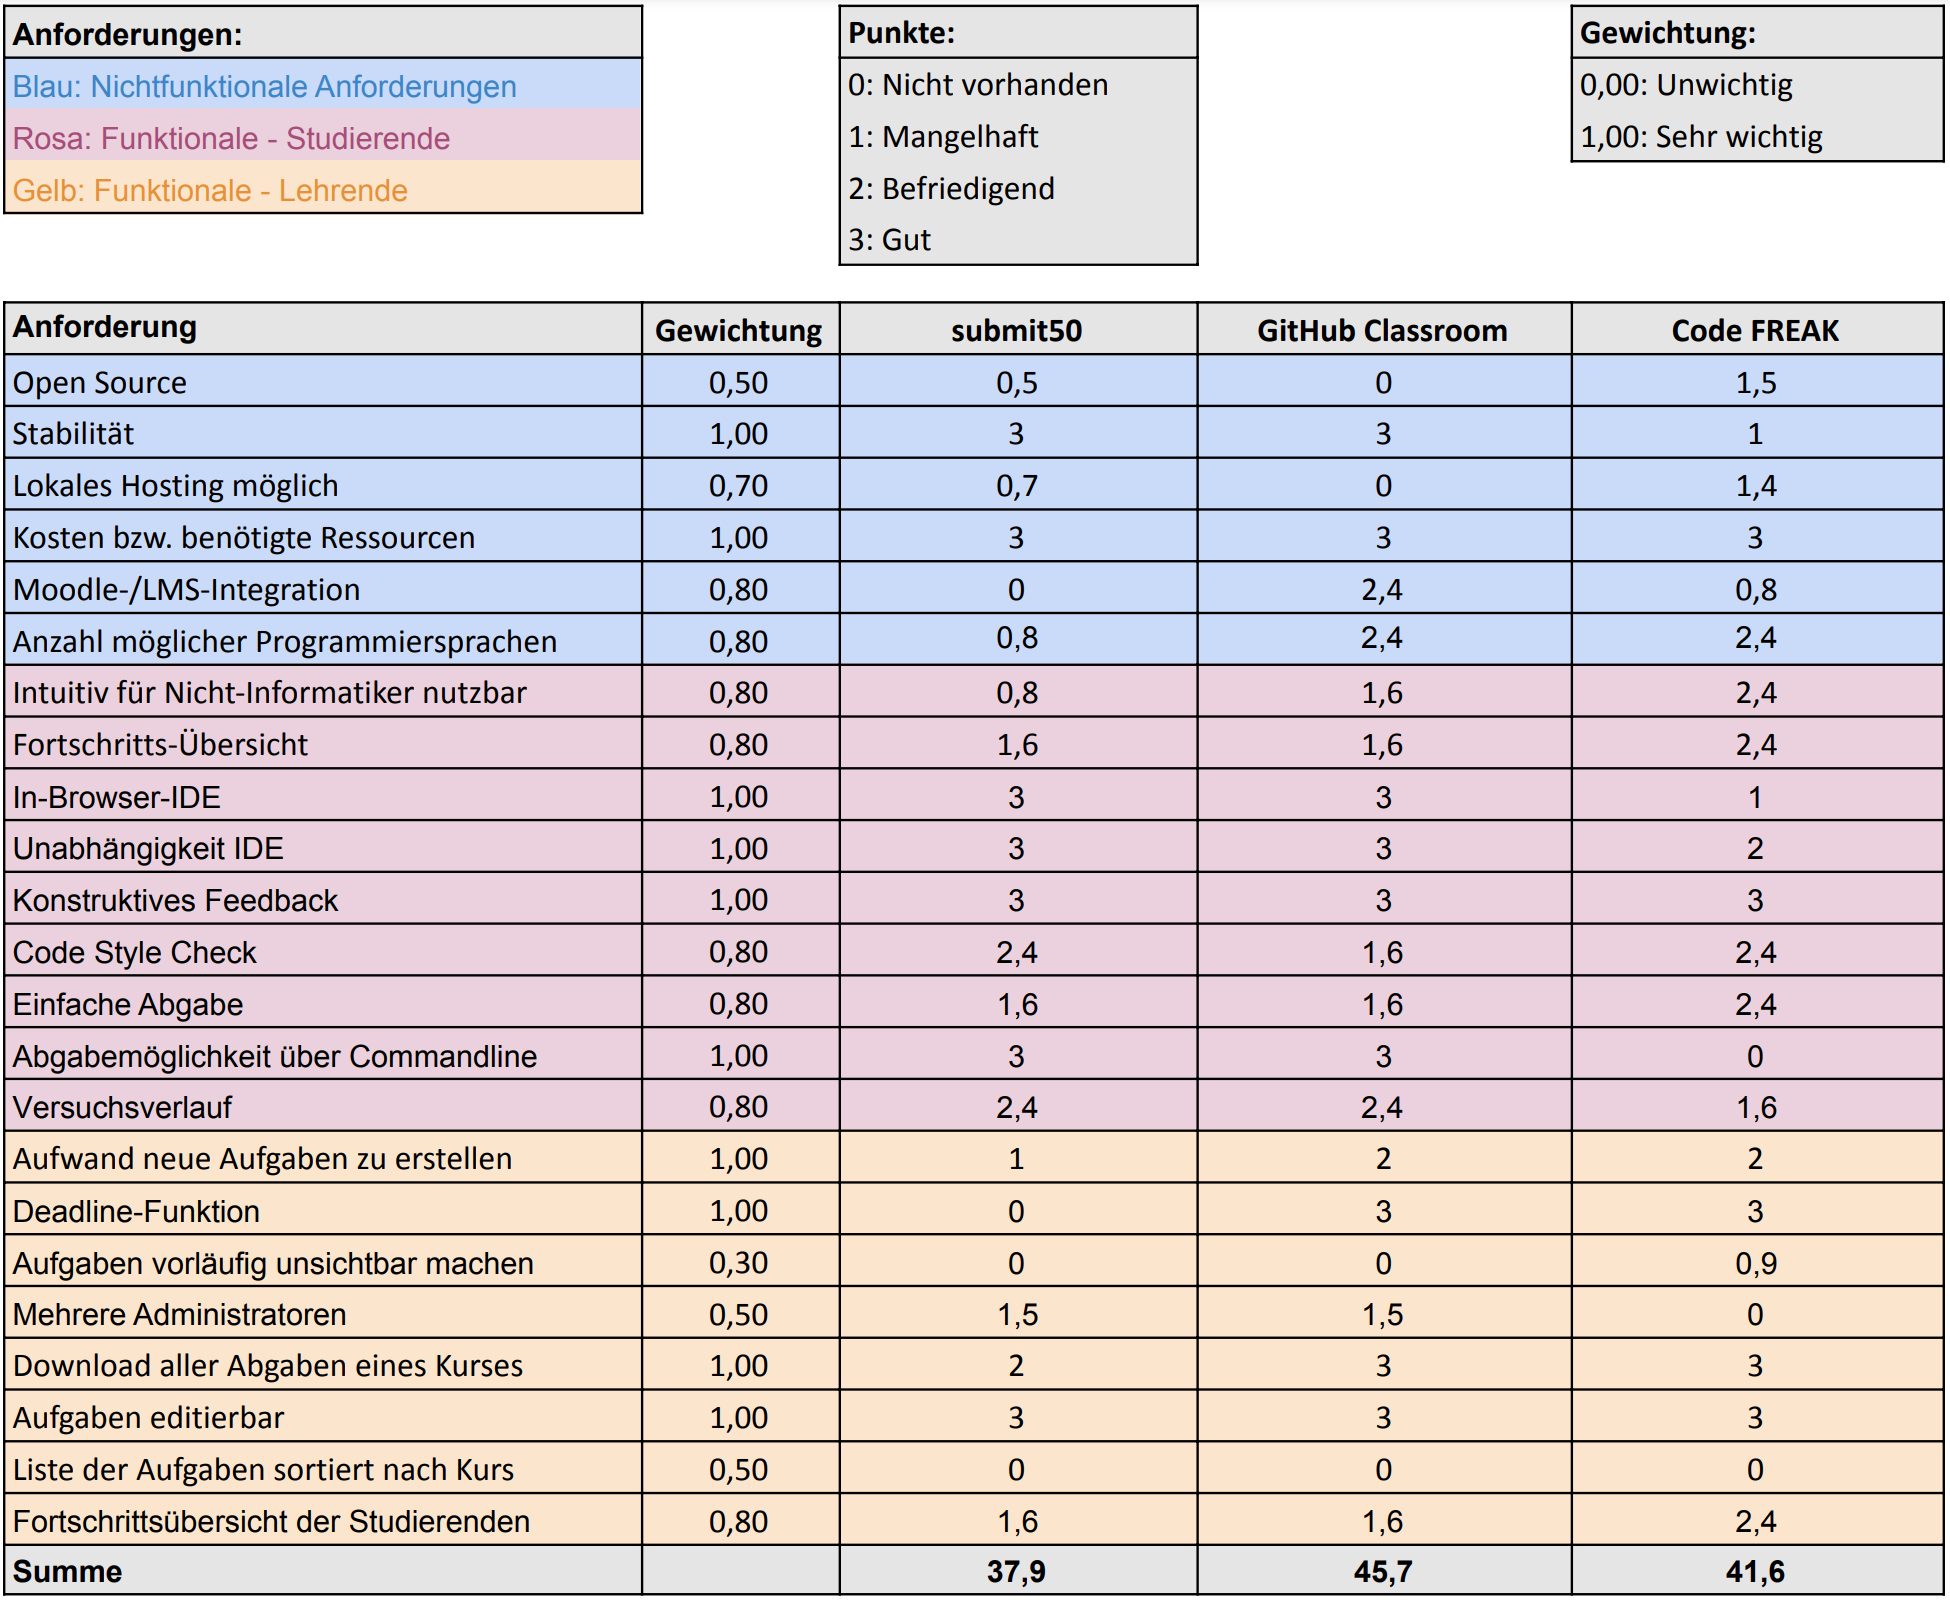
\includegraphics[width=\textwidth]{systemvergleich}
    \caption{Vergleich und Benotung der Systeme}
    \bildquelle{Eigene Darstellung}
    \label{fig:systemvergleich}
\end{figure}

Zusammenfassend befinden sich in der letzten Zeile der Tabelle die Summen der Benotungen. In diesem Fall hat das System mit GitHub Classroom die meisten
Punkte erreicht und wird somit als geeigneter Kandidat für die
Programmierplattform des Zusatzstudiums Digital Skills weiter evaluiert.